\chapter{Конструкторская часть}

\section{Концептуальный дизайн}
Для создания функциональной модели портала, отражающей его основные функции и потоки информации наиболее наглядно использовать нотацию IDEF0. На рисунке \ref{fig:idef0-0} приведена концептуальная модель системы. На рисунке \ref{fig:idef0-1} представлена детализированная концептуальная модель системы в нотации IDEF0.

\begin{figure}[h!]
	\begin{center}
		{\includegraphics[scale = 0.5, angle=0]{../img/idef0/idef0-0.png}}
		\caption{Концептуальная модель системы в нотации IDEF0}
		\label{fig:idef0-0}
	\end{center}
\end{figure}


\begin{figure}[h!]
	\begin{center}
		{\includegraphics[scale = 0.4, angle=90]{../img/idef0/idef0-1.png}}
		\caption{Детализированная концептуальная модель системы в нотации IDEF0}
		\label{fig:idef0-1}
	\end{center}
\end{figure}


\clearpage
\section{Сценарии функционирования системы}

\textbf{Регистрация пользователя}
\begin{enumerate}
	\item Пользователь нажимает на кнопку <<Войти>> в интерфейсе.
	\item Так как у пользователя нет аккаунта, он нажимает на кнопку <<Зарегистрироваться>>.
	\item Пользователь перенаправляется на страницу, которая содержит поля для заполнения его данных.
	\item Пользователь вводит данные в форму и для завершения регистрации нажимает на кнопку <<Готово>>, тем самым подтверждая верность своих данных, а также согласие на их обработку и хранение.
	\item Если пользователь с введенным для регистрации логином, почтой или номером телефона уже существует, то клиент получает сообщение об ошибке. При успешной регистрации клиент попадает на главную страниицу сайта.
\end{enumerate}

\textbf{Авторизация клиента}
\begin{enumerate}
	\item Пользователь нажимает на кнопку <<Войти>> в интерфейсе.
	\item Пользователь перенаправляется на страницу авторизации, которая содержит поля для заполнения логина и пароля.
	\item Пользователь завершает работу с формой авторизации нажатием кнопки <<Готово>>.
	\item При обнаружении ошибки в данных, пользователь получает сообщение об ошибке; при совпадении данных с записью в базе данных аккаунтов пользователь получает доступ к системе и перенаправляется на гланый экран сайта.
\end{enumerate}

\textbf{Оформление аренды книги}
\begin{enumerate}
	\item Пользователь на главной странице видит список всех библиотек. При желании он может отфильтровать их по городу расположения.
	\item Пользователь нажимает на кнопку <<Посмотреть книги>> у понравившейся библиотеки.
  \item Пользователь выбирает книгу в выбранной библиотеке и нажимает кнопку <<Забронировать>>.
	\item Пользователь попадает на страницу, на которой он видит полную информацию о выбранной библиотеке, выбранной книге. Там же ему нужно ввести дату возврата книги и подтвердить согласие с правилами сайта.
	\item Если все верно и пользователь ввел все данные, он нажимает на кнопку <<Готово>>. Если же книга в момент аренды не закончилась в библиотеке, пользователь аутентифицирован и его рейтинг больше, чем количество уже арендованных книг, то он получает соответсвующее сообщение об ошибке. Иначе книга попадает в список забронированных.
\end{enumerate}

\textbf{Возврат книги из аренды}
\begin{enumerate}
	\item Пользователь нажимает на иконку профиля.
	\item Ему выпадает список вкладок сайта, доступных аутентифицированному пользователю.
  \item Пользователь нажимает на вкладку <<Бронирования>>.
	\item Пользователь попадает на страницу, на которой он видит все свои аренды книг. Есть возможность отфильтровать по статусу бронирования.
	\item Пользователь выбирает аренду, котороую он хочет завершить и нажимает на соответсвующее окно бронирования.
	\item Пользователь получает информацию о библиотеке, в которой эта книга арендована, и информацию о самой книге, а также о датах взятия книги в аренду и дате возврата.
  \item Пользователь нажимает на кнопку <<Вернуть книгу>> и получает модалньое окно, в котором необходимо ввести состояние книги и согласиться с правилами сайта.
  \item Если пользователь вернул книгу в более плохом состоянии, чем она была или позже срока, то за каждое условие он получит минус 10 к рейтингу, что уменьшит количество книг, которое он сможет арендовать в дальнейшем. Иначе пользователь получит плюс 1 к рейтингу.
  \item Затем пользователь увидит, что статус аренды книги изменился на <<Возвращена в срок>> или <<Возвращена после срока>>.
\end{enumerate}


\section{Диаграммы прецедентов}
В системе выделены 3 роли: Неавторизованный пользователь, Авторизованный пользователь, Администратор. На рисунках \ref{fig:use-case-non-auth}-\ref{fig:use-case-admin} представлены диаграммы прецедентов для каждой из ролей.

\begin{figure}[H]
	\begin{center}
		{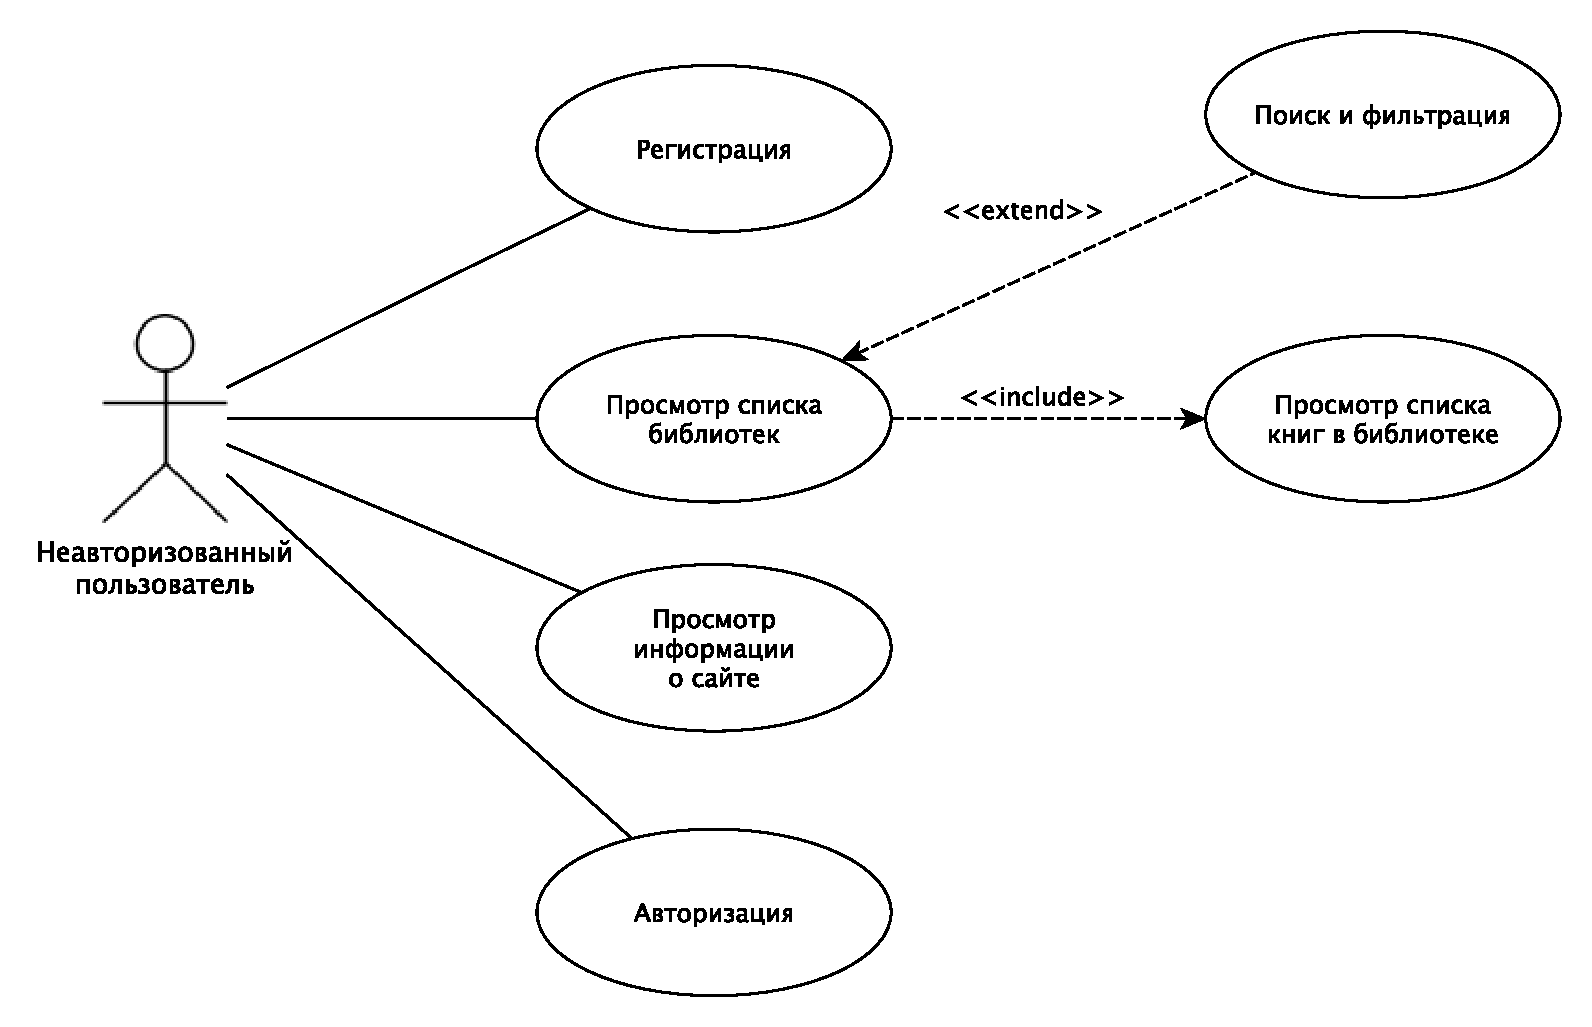
\includegraphics[scale = 0.5]{../img/use-case/non-auth-user.pdf}}
		\caption{Диаграмма прецедентов с точки зрения Неавторизованного пользователя}
		\label{fig:use-case-non-auth}
	\end{center}
\end{figure}

\begin{figure}[H]
	\begin{center}
		{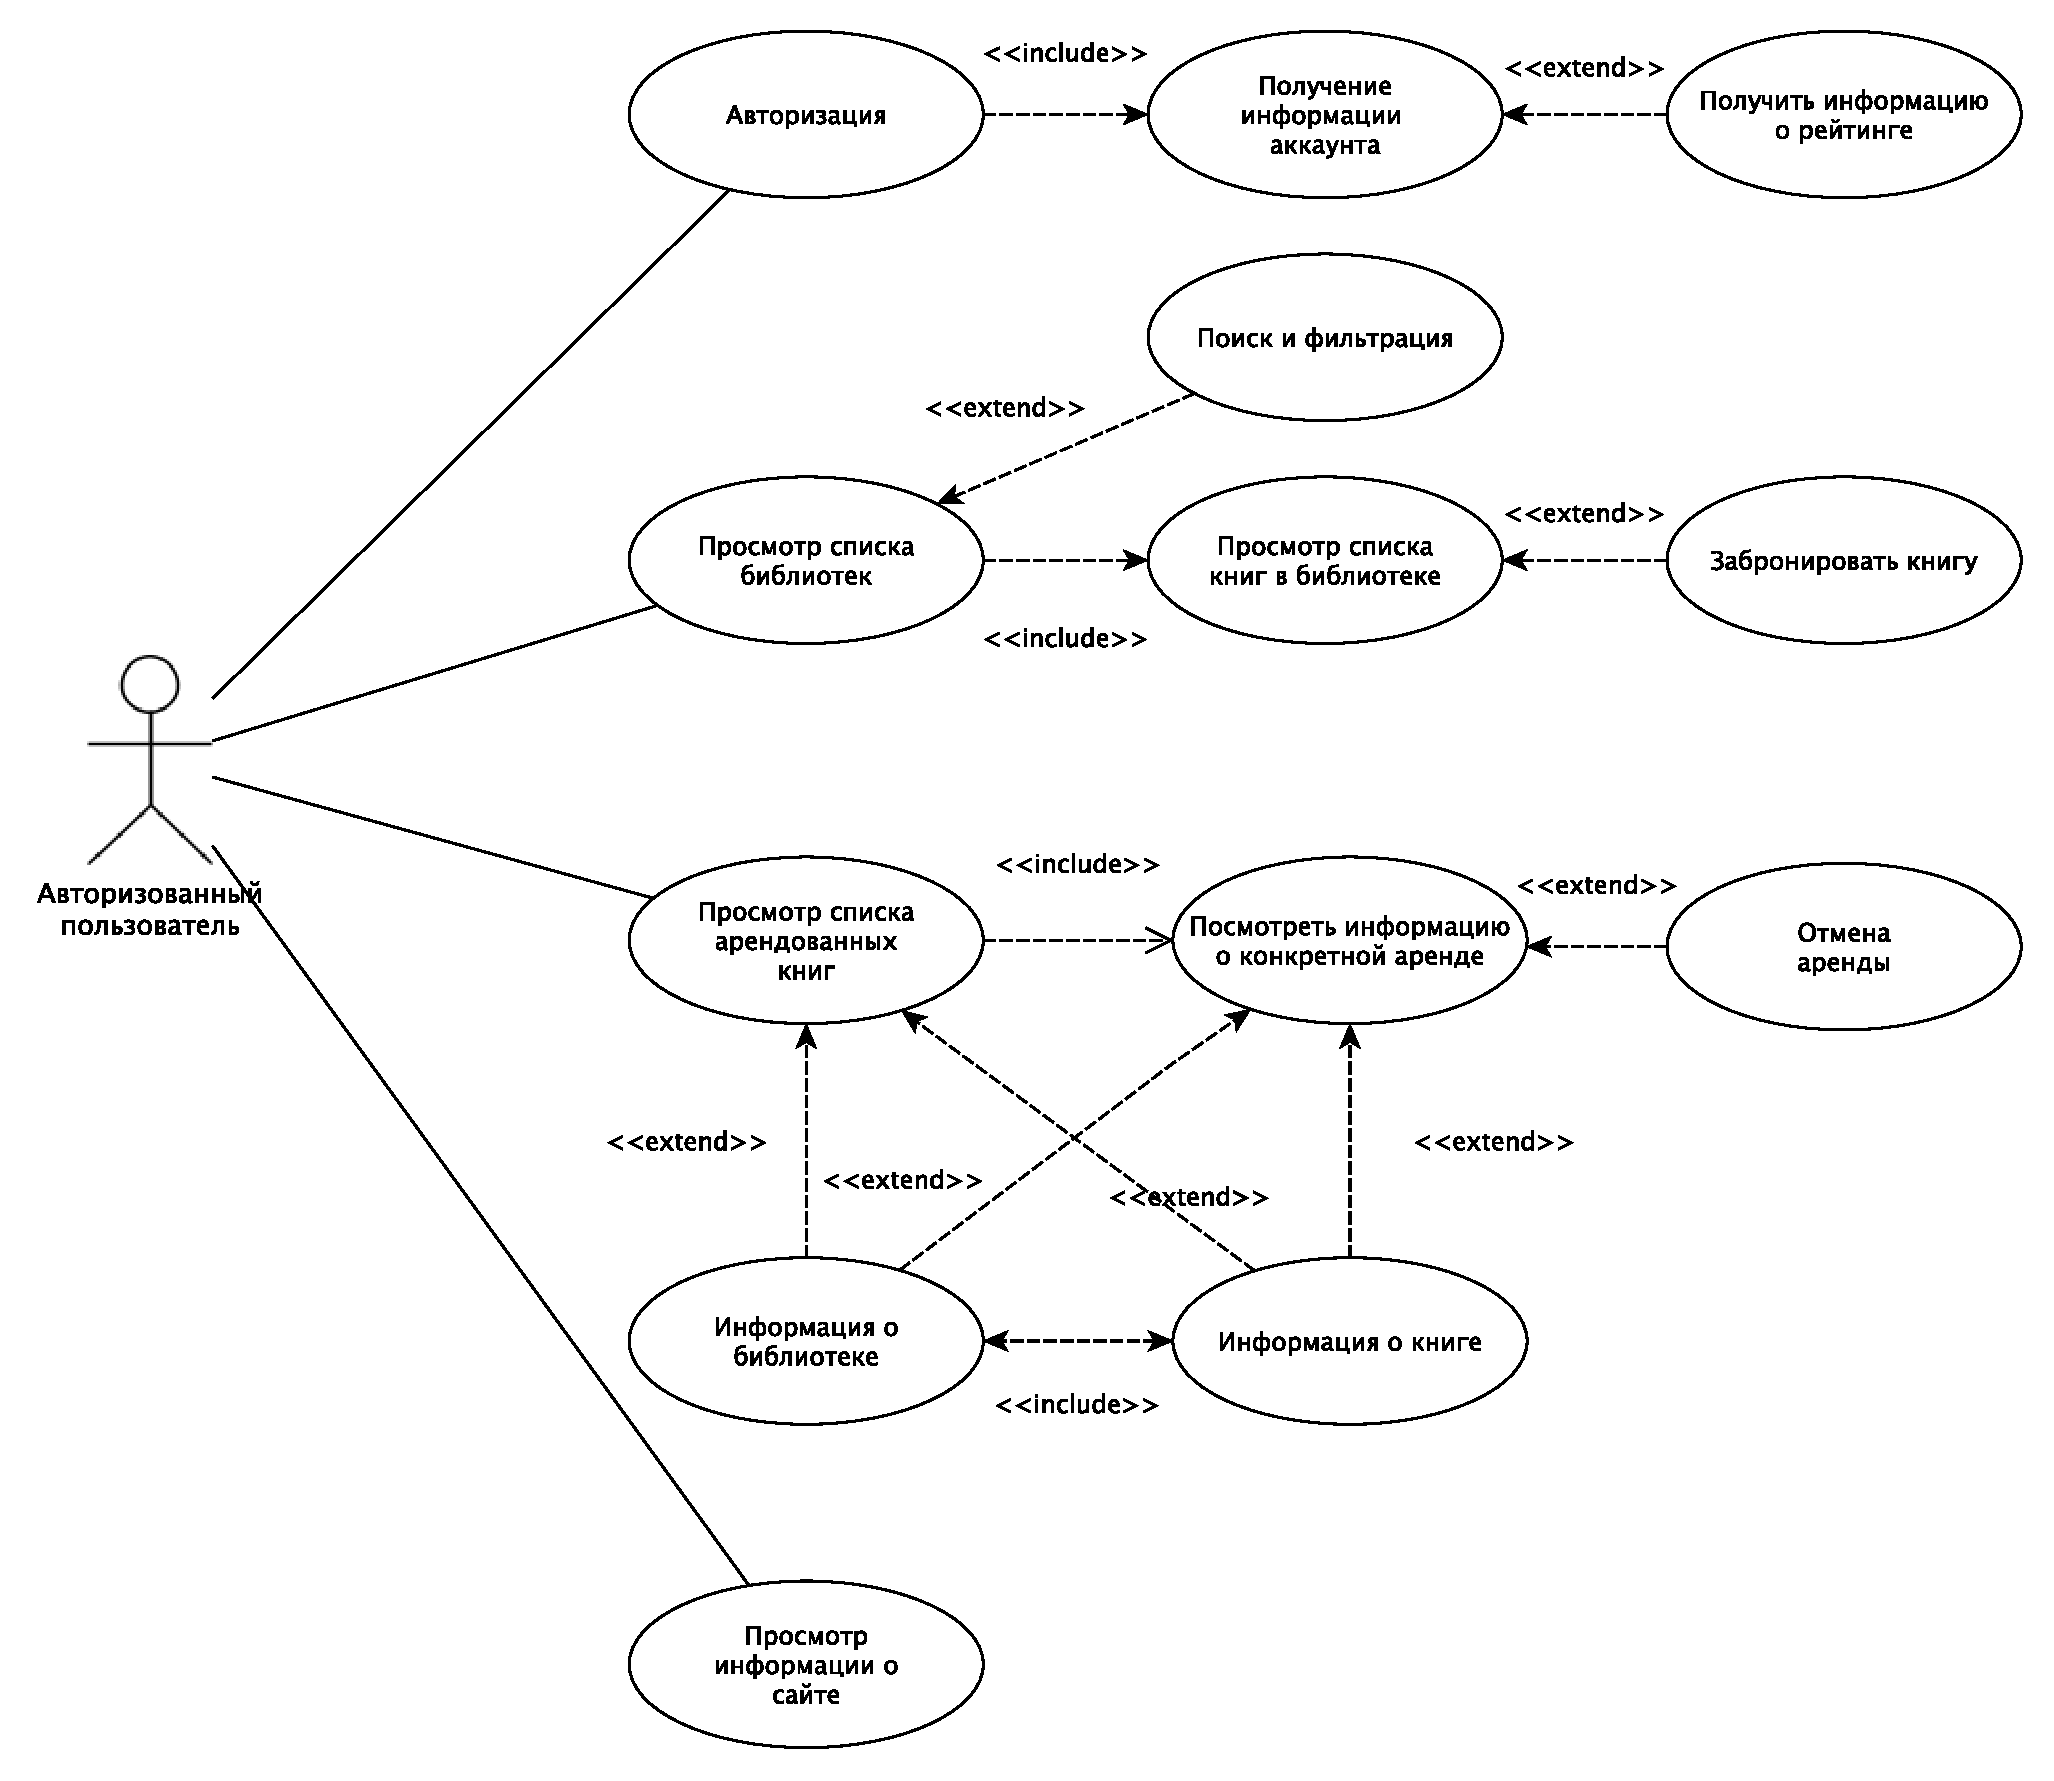
\includegraphics[scale = 0.4]{../img/use-case/auth-user.pdf}}
		\caption{Диаграмма прецедентов с точки зрения Авторизованного пользователя}
		\label{fig:use-case-auth}
	\end{center}
\end{figure}

\begin{figure}[H]
	\begin{center}
		{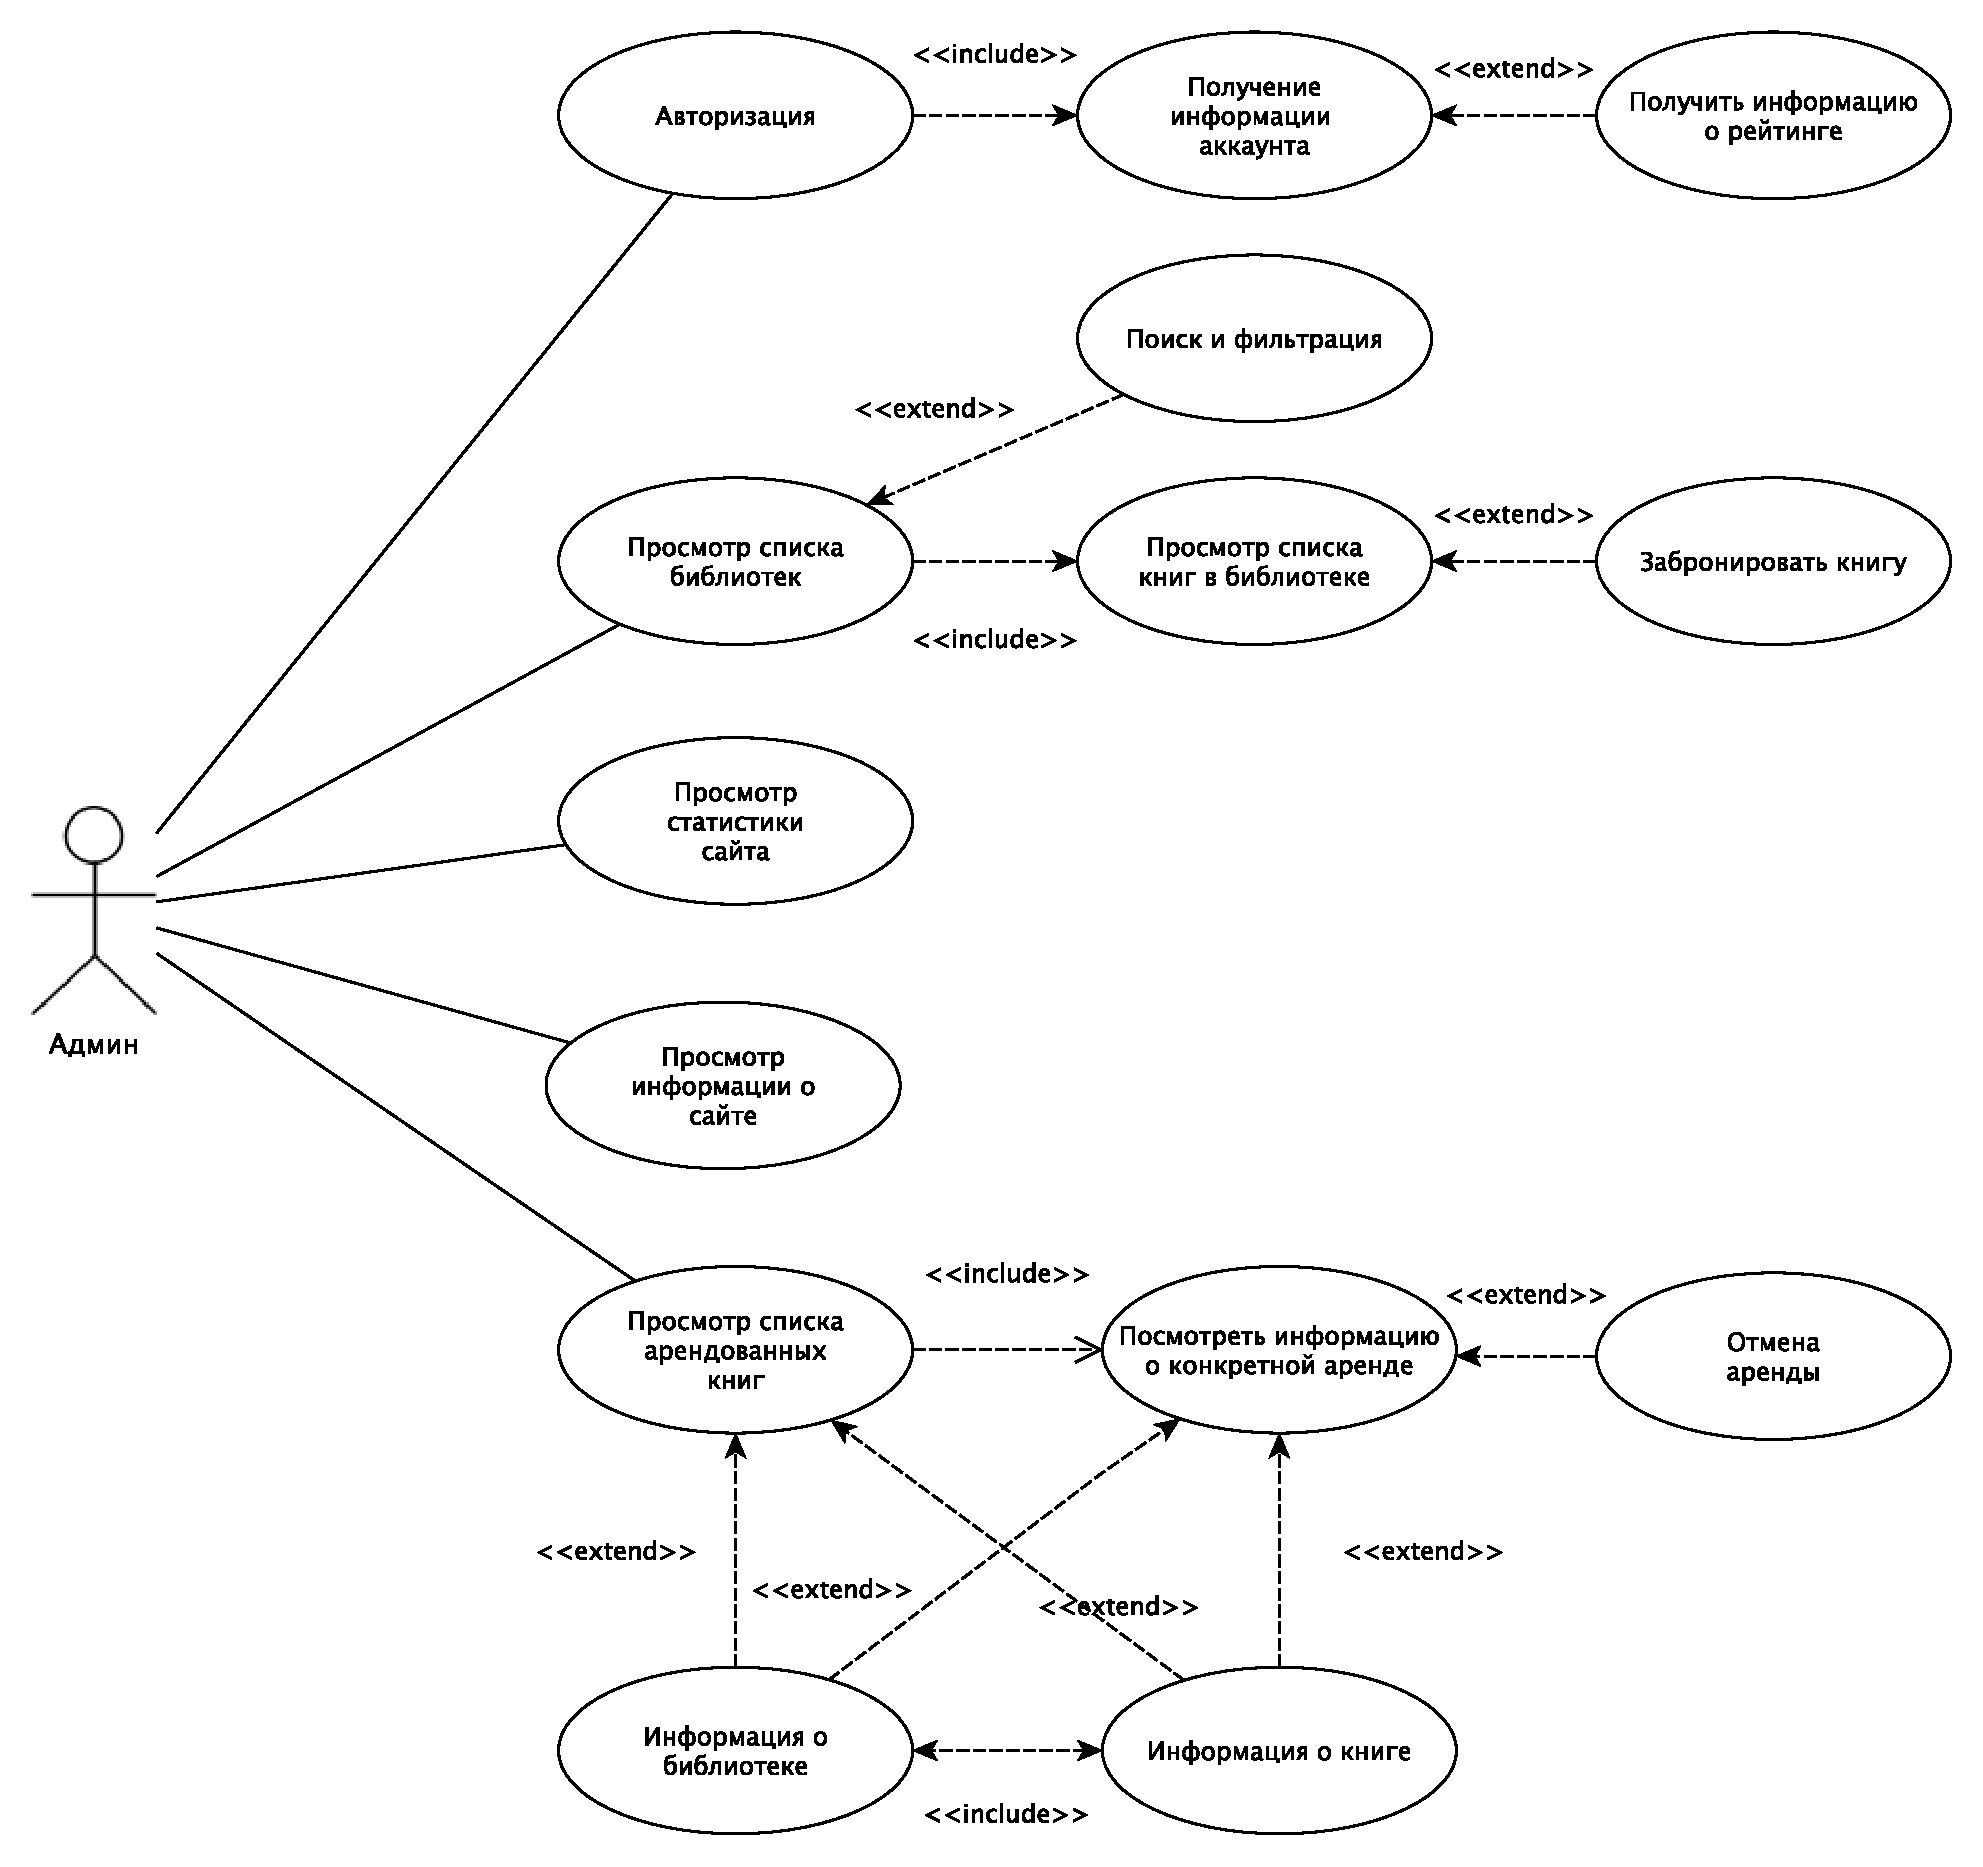
\includegraphics[scale = 0.4]{../img/use-case/admin.pdf}}
		\caption{Диаграмма прецедентов с точки зрения Администратора}
		\label{fig:use-case-admin}
	\end{center}
\end{figure}


\section{Высокоуровневый дизайн пользовательского интерфейса}

Пользовательский интерфейс в разрабатываемой системе представляет собой web-интерфейс, доступ к которому осуществляется через браузер (тонкий клиент). Страница системы состоит из <<шапки>>, основной части.  

Обобщенно структуру страниц системы можно представить следующим образом:
\begin{itemize}
  \item страница авторизации;
	\item страница регистрации;
	\item главная страница со списком библиотек и информацией о каждой из них;
	\item страница со списком книг и информацией о каждой из них;
	\item страница с арендой книги;
	\item страница со всеми арендованными книгами;
	\item страница о сайте с правилами и контактной информацией.
\end{itemize}

Также на рисунках \ref{fig:design-main}-\ref{fig:design-all-reservs} приведены для примеры страниц: <<Главная>>, <<Авторизация>>, <<Бронирование книги>> и <<Все бронирования>>.

\begin{figure}[H]
	\begin{center}
		{\includegraphics[scale = 0.25]{../img/design/main.png}}
		\caption{Главная страница}
		\label{fig:design-main}
	\end{center}
\end{figure}

\begin{figure}[H]
	\begin{center}
		{\includegraphics[scale = 0.25]{../img/design/login.png}}
		\caption{Страница авторизации}
		\label{fig:design-auth}
	\end{center}
\end{figure} 

\begin{figure}[H]
	\begin{center}
		{\includegraphics[scale = 0.25]{../img/design/reserv.png}}
		\caption{Страница бронирования книги}
		\label{fig:design-reserv}
	\end{center}
\end{figure}

\begin{figure}[H]
	\begin{center}
		{\includegraphics[scale = 0.25]{../img/design/all-reservs.png}}
		\caption{Страница со всеми забронированными книгами}
		\label{fig:design-all-reservs}
	\end{center}
\end{figure}
